\subsection{Komponentbeskrivning}

\begin{figure}
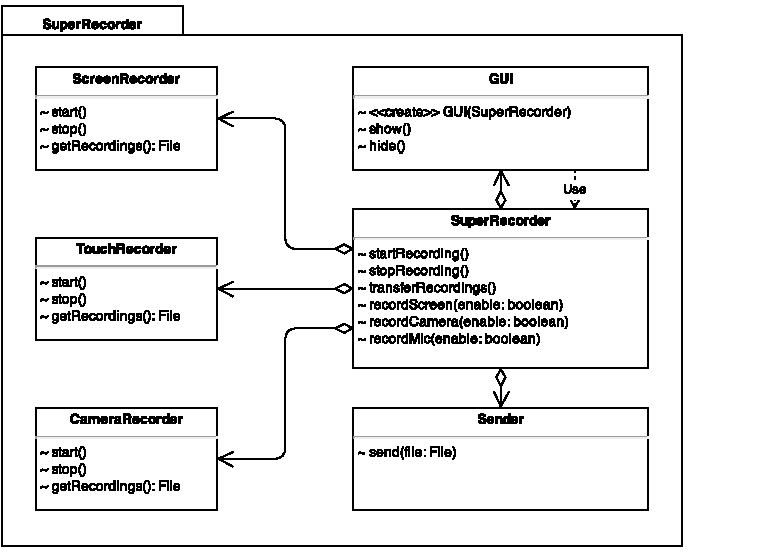
\includegraphics{CrudeClassDiagram.pdf}
\caption{Klassdiagram}
\label{fig:CrudeClassDiagram}
\end{figure}

SuperRecorder-SDK:t är utformat enligt \ref{fig:CrudeClassDiagram}. \\

Klassen SuperRecorder är den centrala klassen i SDK:t och behåller primär kontroll under hela SDK:ts scope. SuperRecorder-klassen initialiserar samtliga andra moduler inom SDK:t och all intern kommunikation inom SDK:t förmedlas via denna klass. \\

GUI:t är den primära möjligheten för extern kommunikation till SDK:t. Genom GUI:t kan användaren ändra inställningar, starta/stoppa inspelning samt sända inspelning till servern. \\

ScreenRecorder ansvarar för inspelning av de aktiviteter som utförs av test-applikationen. Klassen sparar inspelningen i form av en fil som kan returneras vid förfrågan från SuperRecorder-klassen. SuperRecorder-klassen kan även begära start/stopp av inspelning. I övrigt har ScreenRecorder inga publika/package metoder. \\

TouchRecorder ansvarar för dokumentering av touch relevanta till de aktiviteter som utförs av test-applikationen. I övrigt är klassen extern sett att likställa med ScreenRecorder. \\

CameraRecorder ansvarar för inspelning av frontkameran och dess mikrofon under körning av test-applikationen. I övrigt är klassen extern sett att likställa med ScreenRecorder. \\

Sender sköter överföringen av media-filen till servern. \\

På servern konverteras media-filen till lämpligt format för lagring och uppspelning.
